\documentclass{beamer}

\usepackage{pgfpages}
% for presentation on two beamers
\setbeameroption{second mode text on second screen=left}
% \setbeameroption{show notes on second screen}

\usetheme{Darmstadt}

\usecolortheme{beaver}

\usefonttheme[onlymath]{serif}

\usepackage{lmodern}
\usepackage[T1]{fontenc}
\usepackage[utf8]{inputenc}
\usepackage[ngerman]{babel}

\usepackage{hyperref}
\usepackage{caption}
\usepackage{csquotes}

\usepackage[backend=biber,style=numeric,sorting=none,url=false]{biblatex}
\addbibresource{literatur.bib}

\usepackage{array}
\usepackage{mathtools}

\usepackage{stmaryrd} % for contradiction lightning symbol

\usepackage{tikz}
\usetikzlibrary{automata, positioning}
\tikzset{
    state/.style={rounded corners=3pt, minimum width=35pt, draw},
    initial text={},
    shorten >= 1pt,
    every label/.style={font=\scriptsize}
}


\beamertemplatenavigationsymbolsempty
\newcounter{slideinframe}
\defbeamertemplate*{footline}{slide in frame number}{%
    \hfill%
    \usebeamercolor[fg]{page number in head/foot}%
    \usebeamerfont{page number in head/foot}%
    \ifnum\insertframeendpage>\insertframestartpage
        \setcounter{slideinframe}{\numexpr\thepage-\insertframestartpage+1}
        \insertframenumber{}\,-\,\theslideinframe
    \else
        \insertframenumber{}
    \fi%
    %\;/\;\inserttotalframenumber
        \kern1em\vskip2pt%
}


\DeclareMathOperator{\Paths}{Paths}
\DeclareMathOperator{\trace}{trace}
\DeclareMathOperator{\Traces}{Traces}
\DeclareMathOperator{\Post}{Post}
\DeclareMathOperator{\pref}{pref}
\DeclareMathOperator{\closure}{closure}



\begin{document}

\title[Decomposition Theorem]{Dekomposition von Linear-Time Properties}
\author{Stefan Walter}
\institute{Universit"at Leipzig}
\date{\today}

\frame[typeset second]{\only<second:0>{\titlepage}}

\begin{frame}{Literatur}
    \printbibliography
\end{frame}

\begin{frame}{Motivation}
    \begin{center}
        \usetikzlibrary{arrows}
        \begin{tikzpicture}[
            part/.style = {draw, thick, minimum width=40pt}
        ]
        \node[part] (sys)                      {System};
        \node[part] (ts)  [below=2 of sys]     {Transitions-System};

        \node[part] (eig) [right=4 of sys]     {Eigenschaft};
        \node[part] (ltp) [below=2 of eig]     {Linear-Time-Property};

        \path[->, every node/.style={sloped,anchor=south,font=\small}]
                    (ts)  edge node{modelliert} (sys)
                    (ltp) edge node{modelliert} (eig);

        \draw[implies-implies, double equal sign distance,shorten >= 1cm, shorten <= 1cm] (sys) -- (eig);
        \end{tikzpicture}
    \end{center}
\end{frame}




\section{Transitions-Systeme}



\subsection{Einstieg}

\newcommand{\deftranssys}{
    \begin{Definition}[Transitions-System $TS$]
        $TS = (S, Act, \rightarrow, I, AP, L)$ mit:
        \begin{itemize}
            \setlength{\itemindent}{2.5cm}
            \item[$S$] Menge von Zust"anden (States)
            \item[$Act$] Menge von Aktionen (Actions)
            \item[$\rightarrow \; \subseteq \;  S \times Act \times S$] Transitions- ("Ubergangs-) Relation
            \item[$I \subseteq S$] Menge von initialen Zust"anden
            \item[$AP$] Menge von atomaren Aussagen \\ \hspace{5cm} (atomic propositions)
            \item[$L: S \rightarrow 2^{AP}$] Labeling-Funktion
        \end{itemize}
    \end{Definition}
}

\begin{frame}{Transitions-System}
    \deftranssys

    Bemerkungen:
    \begin{itemize}
        \item TS \alert{endlich}, gdw. S, Act und AP endlich
        \item Notation: $s \overset{\alpha}{\rightarrow} s'$ gdw. $(s,\alpha,s') \in \rightarrow$
    \end{itemize}



    \note{$2^{AP}$ bezeichnet die Potenzmenge von $AP$}
    \note{$L$ weist einem Zustand bestimmte Eigenschaften zu}
    \note{nichtdeterministische Wahl bei mehreren init. Zust"anden/Transitionen}
    \note{$AP$ bekannt aus Aussagenlogik}
    \note{f"ur aussagenlogisch Formel $\Phi$: $s \models \Phi$ gdw. $L(s) \models \Phi$}

    \note{Vergleich $TS = (S, Act, \rightarrow, I, AP, L)$ und
            endlicher Automat $\mathcal{A} = (Q,T,I,F)$ "uber Alphabet A:
            "ahnlich:
            \begin{itemize}
                \item $S$ und $Q$
                \item $Act$ und $A$  \\
                    anderer Ansatz, erweiterbares Model: Kommunikation/Synchronisation ueber Aktionen (gleicher Name), Program Graphs
                \item $\rightarrow$ und $T$
                \item Initialzust"ande $I$
            \end{itemize}

            unterschiedlich
            \begin{itemize}
                \item Finalzust"ande (Annahme parallele Systeme laufen ohne Ende)
                \item Alphabete: einmal $\Sigma$ und einmal $AP$/$L$
            \end{itemize}}
\end{frame}

\newcommand{\ampel}{
    \begin{tikzpicture}
        \node[state] (r)                 {rot};
                \draw[->] ++(-3em,0) -- (r);
        \node[state] (g) [below=of r, label=below:\{fahren\}]  {gr"un};

        \path[->]   (r) edge [bend left] node[right]{r-g} (g)
                                (g) edge [bend left] node[left]{g-r}  (r);
    \end{tikzpicture}
}

\begin{frame}[typeset second]{Beispiele TS - Ampel}
    \only<second>{\frametitle{Transitions-System} \deftranssys}

    \only<second:0>{
        \begin{Beispiel}[vereinfachte Ampel]
            $TS_{Ampel} = (S, Act, \rightarrow, I, AP, L)$ mit:

            \begin{columns}
                \column {0.6\textwidth}
                    \begin{itemize}
                        \setlength{\itemsep}{1em}
                        %\item $S = \{ \text{rot, gr"un} \}$
                        \item $Act = \{ \text{r-g, g-r} \}$
                        %\item $\rightarrow\; = \{ (\text{rot}, \text{r-g}, \text{gr"un}),
                        %                                               (\text{gr"un}, \text{g-r}, \text{rot}) \}$
                        %\item $I = \{ \text{rot} \}$
                        \item $AP = \{ \text{fahren} \}$
                        %\item $L = \{ (\text{rot}, \emptyset), (\text{gr"un}, \{ \text{fahren} \}) \}$
                    \end{itemize}

                \pause

                \column{0.35\textwidth}
                    \ampel
            \end{columns}
        \end{Beispiel}

        \note{Wahl von S/Act/AP nicht eindeutig/trivial}
        \note{oft l"asst man einiges weg, z.\,B.
            Labels (oft implizit: $AP = S$ und $L(s) = \{s\}$) und
            Aktionsnamen (nur Kommunikation/Synchronisation)}
    }
\end{frame}



\subsection{Verhalten von Transitions-Systemen}

\begin{frame}{Nachfolger}
    \begin{Definition}[Nachfolger]
        $TS = (S, Act, \rightarrow, I, AP, L)$ und $s \in S$ \\
        Definiere:
        $$\Post(s) = \Big\{s' \in S \; | \; \exists \alpha \in Act.\; s \overset{\alpha}{\rightarrow} s' \Big\}$$
    \end{Definition}

    \pause

    \begin{Beispiel}
        \begin{columns}
            \column{0.4\textwidth}
                \begin{center}
                    \ampel
                \end{center}

            \column{0.5\textwidth}
                \begin{itemize}
                    \setlength{\itemsep}{1em}
                    \item $\Post(\text{rot}) = \{\text{gr"un}\}$
                    \item $\Post(\text{gr"un}) = \{\text{rot}\}$
                \end{itemize}
        \end{columns}
    \end{Beispiel}
\end{frame}

\begin{frame}{Terminal State}
    % evtl. add whole definition of Post(...)
    \begin{Definition}[Terminal State - Endzustand] % Definition 2.4
        $TS = (S, Act, \rightarrow, I, AP, L)$ und $s \in S$ \\[\baselineskip]
        Definiere:
        $s$ hei"st \alert{Terminal State}
        gdw. $\displaystyle\Post(s) = \emptyset$
    \end{Definition}
\end{frame}

\begin{frame}[typeset second]
    \only<second>{
        \frametitle{Pfade und Traces - Beispiel}

        \begin{columns}
            \column{0.25\textwidth}
                \ampel

            \column{0.75\textwidth}
                \begin{itemize}
                    \setlength{\itemsep}{1em}
                    \item $\pi = \Big(\text{rot gr"un}\Big)^\omega$
                    \onslide<2->{\alert{maximal, $\pi \in \Paths(\text{rot})$}} \\
                    \onslide<3->{$\trace(\pi) = \Big(\{\}\{\text{fahren}\}\Big)^\omega$} \\
                    \onslide<4->{\alert{$\in \Traces(\text{rot})$, \quad $\in \Traces(TS_{Ampel})$}}

                    \item $\hat{\pi} = \text{gr"un rot gr"un}$ \\
                    \onslide<3->{$\trace(\hat{\pi}) = \{\text{fahren}\}\{\}\{\text{fahren}\}$}
                \end{itemize}
        \end{columns}
    }

    \only<second:0>{
        \only<-2>{
            \frametitle{Pfade - Definition}
            \begin{Definition}[Pfadfragment] % Definition 3.4.
                $TS = (S, Act, \rightarrow, I, AP, L)$

                \alert{Unendliches Pfadfragment} $\pi = s_0s_1\dots \; \in S^\omega$:
                    \note{$\omega$ bezeichnet \alert{unendliche} W"orter}
                    $$\text{mit } \forall i > 0.\; s_i \in \Post(s_{i-1})$$

                \alert{Endliches Pfadfragment} $\hat{\pi} = s_0s_1\dots s_n \; \in S^*$, \quad $n\geq 0$:
                    $$\text{mit } \forall 0 < i \leq n.\; s_i \in \Post(s_{i-1})$$

                \pause

                \alert{Maximales Pfadfragment} $\pi_{max}$: \\ \hspace{2cm} $\hat{\pi}$ mit Terminal State $s_n$; \; oder $\pi$
                    % \\ \hfill entweder unendlich, oder endlich und endet in Terminal State
                    \\[\baselineskip]

                    \note{entweder endlich und endet in Terminal State; oder unendlich}
                    \note{kann nicht mehr verl"angert werden}

                F"ur $s \in S$ definiere:
                    $\alert{\Paths(s)} = \{ \pi_{max} \; | \; s_0 = s \}$
                    \note{hier unendlich, da TS ohne Endzustand}
            \end{Definition}
        }

        \only<3->{
            \frametitle{Traces - Definition}
            \begin{Definition}[Trace und Trace-Fragment]% Definition 3.8.
                $TS = (S, Act, \rightarrow, I, AP, L)$ ohne Terminal States
                \begin{itemize}
                    \item unendliches Pfadfragment $\pi = s_0s_1\dots \in S^\omega$
                    \begin{flalign*}
                    &\qquad \text{definiere: } \quad \alert{\trace(\pi)} = L(s_0)L(s_1)\dots \in (2^{AP})^\omega&
                    \end{flalign*}
                    \item endliches Pfadfragment $\hat{\pi} = s_0s_1\dots{}s_n \in S^*$
                    \begin{flalign*}
                    &\qquad \text{definiere: } \quad \alert{\trace(\hat{\pi})} = L(s_0)L(s_1)\dots L(s_n) \in (2^{AP})^*&
                    \end{flalign*}
                \end{itemize}

                \onslide<4->{
                    Erweiterung auf:
                    \begin{itemize}
                        \item Mengen von Pfaden $\Pi$: \quad $\trace(\Pi) = \bigcup_{\pi \in \Pi} \trace(\pi)$
                        \item $s \in S$: \quad $\Traces(s) = \trace\Big(\Paths(s)\Big)$
                        \item $TS$: \quad $\Traces(TS) = \bigcup\limits_{s\in I} \Traces(s)$
                    \end{itemize}
                }
            \end{Definition}
        }
    }
\end{frame}



\section{Linear-Time Properties}

\subsection{Einstieg}

\begin{frame}[typeset second]
    \only<second:0>{
        \frametitle{Linear-Time Property}

        Motivation: Formalisierung Eigenschaften eines TS
        \begin{Definition}[Linear-Time Property $P$ "uber $AP$]% Definition 3.10.
            $$P \subseteq (2^{AP})^\omega$$
        \end{Definition}

        \note{Sprache "uber $2^{AP}$ (mit unendlichen W"ortern); Menge von Traces}
        \note{formalisiert Eigenschaften der Traces einse $TS$}

        \pause

        \begin{Definition}[Erf"ullbarkeit / Verifikation von LT-Properties]% Definition 3.11.
                $TS = (S, Act, \rightarrow, I, AP, L)$ ohne Terminal States; $s \in S$ \\[\baselineskip]
                $TS$ bzw. $s$ \alert{erf"ullt (satisfies)} $P$
                gdw. $$\Traces(TS) \subseteq P \quad \text{ bzw. } \quad \Traces(s) \subseteq P$$

                Notation: $TS \models P$ bzw. $s \models P$
        \end{Definition}

        \note{warum ohne Terminal States}
        \note{Annahme parallele Systeme laufen ohne Ende}
        \note{Modellierung/Umwandlung m"oglich}
    }
\end{frame}



\subsection{Invarianten}

\begin{frame}{Invarianten}
    \note{jeder erreichbare Zustand des TS erf"ullt Eigenschaft}
    \note{Namen erkl"aren: gilt in initialen Zust"anden, invariant unter Transitionen}

    Modellierung von z.\,B. Mutual Exclusion, Deadlock-Freiheit
    \note{Mutual Exclusion: es ist immer maximal ein Prozess in seinem kritischen Teil}
    \note{Deadlock-Freiheit: z.\,B. mehrere Prozesse/Threads warten auf die jeweils anderen => Gesamtsystem steht;
            nie Situation, dass beide auf jeweils anderen warten}

    \note{LTL: immer}

    \begin{Definition}[Invariante $P_{inv}$] % Definition 3.20.
        LT-Property $P_{inv}$ "uber $AP$ ist \alert{Invariante}, gdw.
        \begin{align*}
            \exists \text{ aussagenlogische Formel } &\Phi \text{ "uber } AP. \; \\
            P_{inv} = \Big\{ A_0A_1A_2&\dots \in (2^{AP})^\omega \; | \;
            \forall i \geq 0.\; A_i \models \Phi \Big\}
        \end{align*}
    \end{Definition}
\end{frame}


% https://tex.stackexchange.com/questions/6135/how-to-make-beamer-overlays-with-tikz-node
\tikzset{onslide/.code args={<#1>#2}{%
        \only<#1>{\pgfkeysalso{#2}} % \pgfkeysalso doesn't change the path
}}
\tikzset{temporal/.code args={<#1>#2#3#4}{%
        \temporal<#1>{\pgfkeysalso{#2}}{\pgfkeysalso{#3}}{\pgfkeysalso{#4}} % \pgfkeysalso doesn't change the path
}}

\begin{frame}[typeset second]{Beispiel "Uberpr"ufen von Invarianten - Tiefensuche}% Seite 110
    \only<second> {
        Bemerkung: Algorithmus gilt nur f"ur endliche TS

        \begin{Beispiel}
            \note{zuerst Beispiel zur Verdeutlichung vom Algorithmus;
                danach etwas dazu, wie sinnvoll das ist: eigentlich uninteressant: man modelliert nicht Gesamtsystem sondern Einzelsysteme; =>  Interleaving}

            Ampelkreuzung mit zwei Ampeln und $AP = \{ \text{fahren}_i \}$, \; $i \in \{1,2\}$ \\[\baselineskip]
            In keinem Zustand d"urfen beide Richtungen gleichzeitig fahren.
            $$P_{inv} = \Big\{ \sigma = A_0A_1 ... \in (2^{AP})^\omega \; | \; \forall A_i.\; \{\text{fahren}_1,\text{fahren}_2\} \not \subseteq A_i \Big\}$$
        \end{Beispiel}

        \note{im Text korrekt beschrieben aber im Pseudocode jedoch  falsch formuliert:
                ein pop(U) zuviel => liefert trace fragment bis einen Zustand vor dem, der die Invariante nicht erfuellt}

        $R$ - Menge besuchter Zust"ande \\
        $U$ - Stack; aktuelle Position/Pfad-Fragment \\[\baselineskip]

        eingef"arbt $\in R$ (gr"un [rot]: Invariante gilt [nicht]) \\[\baselineskip]
    }

    \only<second:0>{
        \begin{figure}[h]
            \begin{center}
                \begin{tikzpicture}[
                        node distance=0.6cm,
                        visited/.style={fill=lightgray},
                        good/.style={fill=green},
                        bad/.style={fill=red}
                ]
                    \node[state,onslide=<2->{visited}] (rr)                 {$\text{rot}_1, \text{rot}_2$};
                        \draw[->] ++(0, 2em) -- (rr);
                    \node[state,onslide=<3>{visited},onslide=<4->{good}] (rg) [below left=of rr, label=below:\{$\text{fahren}_2$\}]  {$\text{rot}_1, \text{gr"un}_2$};
                    \node[state,onslide=<5->{visited}] (gr) [below right=of rr, label=above right:\{$\text{fahren}_1$\}] {$\text{gr"un}_1, \text{rot}_2$};
                    \node[state,onslide=<6>{visited},onslide=<7->{bad}] (gg) [below left=1 and 0 of gr, label=below:{\{$\text{fahren}_1, \text{fahren}_2$\}}]
                                                                        {$\text{gr"un}_1, \text{gr"un}_2$};

                    \path[->]   (rr) edge [bend right] (rg)
                                                     edge [bend left]  (gr)
                                            (rg) edge [bend right] (rr)
                                            (gr) edge [bend left]  (rr)
                                                     edge [bend left]  (gg)
                                            (gg) edge [bend left]  (gr);
                \end{tikzpicture}
            \end{center}
            \caption{bewusst falsch modellierte Ampelkreuzung (ohne $Act$)}
        \end{figure}

    \newcommand{\srr}{(\text{rot}_1, \text{rot}_2)}
    \newcommand{\sgr}{(\text{gr"un}_1, \text{rot}_2)}
    \newcommand{\srg}{(\text{rot}_1, \text{gr"un}_2)}
    \newcommand{\sgg}{(\text{gr"un}_1, \text{gr"un}_2)}

    \vspace*{-1em}

        \begin{flalign*}
            &R = \{ \only<2->{\srr} \only<3->{, \srg} \only<5->{, \sgr} \only<6->{\sgg} \}& \\[0.8\baselineskip]
            &U = \$\only<2->{\srr} \only<3>{\srg} \only<5->{\sgr} \only<6->{\sgg}&
        \end{flalign*}
        \let\srr\undefined \let\sgr\undefined \let\srg\undefined \let\sgg\undefined
    }
\end{frame}



\subsection{Safety Properties}

\newcommand{\defpraefix}{
    \begin{definition}[Pr"afix] % Definition 3.26; Praefix von Woertern: S.913 Absatz 2
        Trace $\sigma = A_0A_1A_2\dots \in (2^{AP})^\omega$ und LT-Property $P \subseteq (2^{AP})^\omega$ \\[\baselineskip]
        Definiere:
        \begin{itemize}
            \item $\pref(\sigma) = \{\hat{\sigma} = A_0A_1\dots A_i \in (2^{AP})^* \; | \; i \geq 0 \}$
            % \text{ ist \alert{endliches} Pr"afix von } \sigma \}$
            % $\pref(\sigma)$ die Menge aller \alert{endlichen Pr"afixe} $\hat{\sigma} \in (2^{AP})^*$ von $\sigma$.
            \item $\pref(P) = \bigcup_{\sigma \in P} \pref(\sigma)$
        \end{itemize}
    \end{definition}
}

\begin{frame}[typeset second]
    \only<second:0>{
        \frametitle{Pr"afix}

        \defpraefix

        \pause

        \begin{Beispiel}[Pr"afix]
            Sei $AP = \{\text{fahren}\}$. \\
            Betrachte $\sigma = (\{rot\}\{gr"un\})^\omega$
            $$\pref(\sigma) = \Big\{\epsilon, \{\}, \{\}\{\text{fahren}\}, \{\}\{\text{fahren}\}\{\}, \dots\Big\}$$
        \end{Beispiel}
    }
\end{frame}

\newcommand{\defsafety}{
    \begin{Definition}[Safety Property $P_{safe}$, Bad Prefixes]% Definition 3.22.
        \note{nach Formulierung "uber eigentlicher Definition im Buch}

        LT-Property $P_{safe}$ "uber $AP$ ist \alert{Safety Property}, gdw.
        $$\forall \sigma \in (2^{AP})^\omega \setminus P_{safe}. \quad \Bigg(
        \exists \hat{\sigma} \in \pref(\sigma). \quad
        \Big( \hat{\sigma} \not\in \pref(P_{safe})\Big)\Bigg)$$

        $\hat{\sigma}$ hei"st \alert{bad prefix f"ur $P_{safe}$}
    \end{Definition}
}

\begin{frame}{Safety Property}
    \defsafety

    \note{Bankautomat: kein Geld abheben ohne Karte}

    $\lnot P_{safe} \implies \exists$ \alert{endliches} Trace-Fragment, das $P_{safe}$ verletzt
    \note{Invarianten sind Safety Properties}
\end{frame}

\begin{frame}[typeset second]{Safety Property - Beispiel}
    \only<second>{\defsafety}

    \only<second:0>{
        \begin{Beispiel}
            Computer mit $AP = \{ \text{an, aus, startet, beendet} \}$ \\[\baselineskip]

            Direkt nach dem Herunterfahren soll der Computer aus sein:
            $$P_{safe} = \Big\{ A_0A_1 ... \; |
                \; \forall A_i.\; \{\text{beendet}\} \subseteq A_i \Rightarrow \{\text{aus}\} \subseteq A_{i+1} \Big\}$$

            Beispiel bad prefix: $\{\text{an}\}\{\text{beendet}\}\{\text{an}\}$
        \end{Beispiel}
    }
\end{frame}



\note{Invarianten sind Safety Properties}
\note{Safety: leicht erf"ullt: System, das nichts macht}
\note{Liveness: gewisse Dinge sollen passieren}



\subsection{Liveness Properties}

\newcommand{\defliveness}{
    \begin{Definition}[Liveness Property $P_{live}$]% Definition 3.33.
        LT-Property $P_{live}$ "uber $AP$ ist \alert{liveness Property}, gdw.
        $$\pref(P_{live}) = (2^{AP})^*$$
    \end{Definition}
}

\begin{frame}[typeset second]
    \only<second>{}

    \only<second:0>{
        \frametitle{Liveness Property}
        Modellierung von z.\,B. \dots (mit $\{ap\} \in AP$)
        \begin{itemize}
            \setlength{\itemsep}{1em}
            \item Eventualit"at:
                    $P = \{ A_0A_1 \dots \enspace | \enspace \exists i \geq 0. \enspace ap \in A_i \}$
            \item wiederholte Eventualit"at: \\
                    $P = \{ A_0A_1 \dots \enspace | \enspace \forall i \geq 0. \enspace \exists j \geq i. \enspace ap \in A_j \}$
        \end{itemize}
        \note{$\exists i \geq 0. \; ap \in A_i$}
        \note{$\forall i \geq 0. \; \exists j > i. \; ap \in A_j$}

        \pause

        \defliveness

        $\lnot P_{live} \implies \exists$ \alert{unendliches} Trace-Fragment, das $P_{live}$ verletzt
    }
\end{frame}



\subsection{Dekompositions-Theorem}

\newcommand{\defclosure}{
    \begin{Definition}[Closure/H"ulle]
        LT-Property $P \subseteq (2^{AP})^\omega$; definiere:
        $$\closure(P) = \big\{ \sigma \in (2^{AP})^\omega \enspace | \enspace \pref(\sigma) \subseteq \pref(P) \big\}$$
    \end{Definition}
}

\newcommand{\lemdistributiveclosure}{
    \begin{Lemma}[Distributivit"at von Vereinigung und $\closure$] %Lemma 3.36.
        $\forall P,P' \subseteq (2^{AP})^\omega$ gilt:
        $$\closure(P) \cup \closure(P') = \closure(P \cup P')$$
    \end{Lemma}
}

\begin{frame}[typeset second]
    \only<second>{
        \defsafety
        \defliveness
    }

    \only<second:0>{
        \defclosure

            \note{Es gibt $P$ mit $\closure(P) \neq P$: w"ahle beliebige Liveness P.
                $\implies$ alternative Definition Safety Property
                        $$\closure(P_{safe}) = P_{safe}$$

                $\implies$ alternative Definition Liveness Property5
                        $$\closure(P_{live}) = (2^{AP})^\omega$$}

        \pause

        $\implies$ alternative Definition f"ur Safety und Liveness: (ohne Beweis)
        $$\closure(P_{safe}) = P_{safe}$$
        $$\closure(P_{live}) = (2^{AP})^\omega$$

        \vfill\pause

        \lemdistributiveclosure
        (ohne Beweis)
    }
\end{frame}

\begin{frame}[typeset second]{Dekompositions-Theorem}
    \only<second>{}

    \only<second:0>{
        Motivation: separate Verifikation einfacher
        \note{Verifikation Safety Property reduziert sich sp"ater auf Invariant Checking}

        \begin{Satz}[Dekomposition von Linear-Time Properties]% Theorem 3.37.
            $\forall P \subseteq (2^{AP})^\omega.
                \enspace \exists P_{safe} \subseteq (2^{AP})^\omega
                    \text{ und } P_{live} \subseteq (2^{AP})^\omega$ \\[0.5\baselineskip]
            $P_{safe}$ ist Safety P. und $P_{live}$ ist Liveness P., sodass

            $$P = P_{safe} \cap P_{live}$$
        \end{Satz}
    }
\end{frame}

\newcommand{\decomposition}{%
    $$P = \underbrace{\closure(P)}_{= P_{safe}} \cap
    \underbrace{\left( P \cup \left( (2^{AP})^\omega \setminus \closure(P) \right) \right)}_{= P_{live}}$$%
}

\newcommand{\venndiagram}{
    \begin{tikzpicture}[thick]
        \draw [rounded corners=0.56cm] (0,0) rectangle (3cm,3cm)  node[below left=3pt]  {$(2^{AP})^\omega$};
        \draw (1.65,0) [rotate=45] ellipse (0.75cm and 1.2cm) node[xshift=3.75, yshift=-0.75em, font=\small] {$\closure(P)$};
        \draw (1.125,1.5) circle (0.22cm) node {$P$};
    \end{tikzpicture}
}

\begin{frame}[typeset second]{Dekompositions-Theorem Beweis}
    \only<second>{
        \defpraefix
        \defclosure
    }

    \only<second:0>{
        \begin{Beweis}
            \begin{columns}
                \column[b]{0.6\textwidth}
                    Sei $P \subseteq (2^{AP})^\omega$ \\~\\
                    Es gilt: $P \subseteq \closure(P) \subseteq (2^{AP})^\omega$
                    \pause

                \column{0.3\textwidth}
                    \venndiagram
            \end{columns}\pause~\\

            \decomposition
        \end{Beweis}
    }
\end{frame}

\begin{frame}[typeset second]{Dekompositions-Theorem Beweis}
    \only<second>{
        \defclosure
        \defsafety
    }

    \only<second:0>{
        \begin{Beweis}
            \decomposition

            \begin{enumerate}[<+->]
                \item zu zeigen: $P_{safe} = \closure(P)$ ist Safety Property
                    \begin{align*}
                        \sigma \in (2^{AP})^\omega \setminus \closure(P)
                        &\iff \pref(\sigma) \not\subseteq \pref(P) \\
                        &\iff \exists \hat{\sigma} \in \pref(\sigma). \; \hat{\sigma} \not\in \pref(P)
                    \end{align*}
            \end{enumerate}
        \end{Beweis}
    }
\end{frame}

\begin{frame}[typeset second]{Dekompositions-Theorem Beweis}
    \only<second>{
        \defclosure
        \defliveness
        \pause
        \lemdistributiveclosure
    }

    \only<second:0>{
        \begin{Beweis}
            \begin{enumerate}
                \setcounter{enumi}{1}
                \item z.z.: $P_{live} = P \cup \left( (2^{AP})^\omega \setminus \closure(P) \right)$ ist Liveness Property \\[\baselineskip]
                    "aquivalente Definition: $\closure(P_{live}) = (2^{AP})^\omega$ \\[\baselineskip]
                    \begin{itemize}[<+->]
                        \item[``$\subseteq$''] $\closure(P_{live}) \subseteq (2^{AP})^\omega$ gilt immer
                        \item[``$\supseteq$'']
                            $\begin{aligned}[t]
                                    \closure(P_{live}) = \closure\Big( P \cup \big( (2^{AP})^\omega \setminus \closure(P) \big) \Big)
                                \end{aligned}$ \\
                            \hfill$\begin{aligned}[t]
                                    &\overset{\mathclap{Distr.}}{=} \qquad \closure(P) \cup \closure\Big( (2^{AP})^\omega \setminus \closure(P) \Big) \\
                                    &\overset{\mathclap{\closure(P')\supseteq P'}}{\underset{\mathclap{\text{Mon. } \cup \text{ bzgl. } \subseteq}}{\supseteq}} \qquad \closure(P) \cup \Big( (2^{AP})^\omega \setminus \closure(P) \Big)
                                = (2^{AP})^\omega
                            \end{aligned}$
                    \end{itemize}
            \end{enumerate}
        \end{Beweis}
    }
\end{frame}










%%%%%%%%%%%%%%%%% %%%%%%%%%%%%%%%%% %%%%%%%%%%%%%%%%% %%%%%%%%%%%%%%%%%
% BACKUP SLIDES % % BACKUP SLIDES % % BACKUP SLIDES % % BACKUP SLIDES %
%%%%%%%%%%%%%%%%% %%%%%%%%%%%%%%%%% %%%%%%%%%%%%%%%%% %%%%%%%%%%%%%%%%%

% https://tex.stackexchange.com/questions/70448/dont-count-backup-slides
\newcommand{\backupbegin}{
    \newcounter{finalframe}
    \setcounter{finalframe}{\value{framenumber}}
}
\newcommand{\backupend}{
    \setcounter{framenumber}{\value{finalframe}}
}


\begin{frame}[typeset second]
    \only<second:0>{
        \Huge\centering Backup Slides
    }
\end{frame}


\newcommand{\lemsharpest}{
    \begin{Lemma}[Sharpest Decomposition]
        LT-Property $P \subseteq (2^{AP})^\omega$ mit $P = P_{safe} \cap P_{live}$. \\[0.5\baselineskip]
        $P_{safe}$ ist Safety P. und $P_{live}$ ist Liveness P. \\

        Es gilt:
        \begin{enumerate}
            \item $\closure(P) \subseteq P_{safe}$
            \item $P_{live} \subseteq P \cup \left( (2^{AP})^\omega \setminus \closure(P) \right)$
        \end{enumerate}
    \end{Lemma}
}

\begin{frame}[typeset second]{Sharpest Decomposition}
    \only<second>{}

    \only<second:0>{
        \lemsharpest
    }
\end{frame}

\begin{frame}[typeset second]
    \only<second>{
        \lemsharpest~\\[\baselineskip]

        \begin{columns}
            \column{0.6\textwidth}
                Wir verwenden: (teilweise ohne Beweis)
                \begin{enumerate}
                    \renewcommand{\theenumi}{\alph{enumi}}
                    \item Monotonie von $\closure$ und $\subseteq$
                    \item alternative Def. Safety
                    \item Monotonie von $\setminus$ und $\subseteq$
                    \item DeMorgan
                \end{enumerate}

            \column{0.3\textwidth}
                \venndiagram
        \end{columns}
    }

    \only<second:0>{
        \begin{Beweis}
            \begin{enumerate}[<+->]
                \item $\begin{aligned}[t]
                        \closure(P) &= \closure(P_{safe} \cap P_{live}) \\
                                                &\overset{a}{\subseteq} \closure(P_{safe})
                                                \overset{b}{=} P_{safe}
                    \end{aligned}$

                \item Widerspruch: Sei $\sigma \not\in P \cup \left( (2^{AP})^\omega \setminus \closure(P) \right)$. \\
                    zu zeigen: $\sigma \not\in P_{live}$

                    $$\begin{aligned}
                        (2^{AP})^\omega \setminus \Big( P \cup &\left( (2^{AP})^\omega \setminus \closure(P) \right) \Big) \\
                                &= \closure(P)\setminus P \\
                                &\overset{1,c}{\subseteq} P_{safe} \setminus (P_{safe} \cap P_{live}) \\
                                &\overset{d}{=} \Big(P_{safe} \setminus P_{safe}\Big) \cup \Big(P_{safe} \setminus P_{live}\Big) \\
                                &= P_{safe} \setminus P_{live}
                    \end{aligned}$$

                    Also $\sigma \not\in P_{live}$. \vspace{-1em}
            \end{enumerate}
        \end{Beweis}
    }
\end{frame}



\begin{frame}[typeset second]
    \only<second>{
        \defpraefix
        \defclosure
    }

    \only<second:0>{
        \begin{Lemma}[Monotonie von $pref$ und $closure$ bzgl. $\subseteq$]
            $\forall P,P' \subseteq (2^{AP})^\omega$ gilt: \quad $P \subseteq P' \implies \dots$
            \begin{enumerate}
                \item $\dots \pref(P) \subseteq \pref(P')$
                \item $\dots \closure(P) \subseteq \closure(P')$
            \end{enumerate}
        \end{Lemma}

        \pause

        \begin{Beweis}
            Annahme: $P \subseteq P'$ \quad \pause also $\forall \sigma \in P. \; \sigma \in P'$ \pause
            \begin{enumerate}[<+->]
                \item trivial: $\begin{aligned}[t] \text{Annahme}
                        &\overset{Def.}{\iff} \forall \sigma \in P. \pref(\sigma) \subseteq \pref(P') \\
                        &\overset{Def.}{\iff} \pref(P) \subseteq \pref(P')
                    \end{aligned}$
                \item $\begin{aligned}[t]
                    \closure(P) &\overset{Def.}{=} \{ \sigma \in (2^{AP})^\omega \enspace | \enspace \pref(\sigma) \subseteq \pref(P) \} \\
                                         &\overset{Ann.}{\underset{1}{\subseteq}}  \{ \sigma \in (2^{AP})^\omega \enspace | \enspace \pref(\sigma) \subseteq \pref(P') \} \\
                                         &\qquad \overset{Def.}{=} \closure(P')
                    \end{aligned}$
            \end{enumerate}
            \vspace*{-1em}
        \end{Beweis}
    }
\end{frame}

\begin{frame}
    \begin{Lemma}[Distributivit"at von Vereinigung und $\pref$]
        $\forall P,P' \subseteq (2^{AP})^\omega$ gilt:
        $$\pref(P) \cup \pref(P') = \pref(P\cup P')$$
    \end{Lemma}

    \begin{Beweis}
        $$\begin{aligned}[t]
                \hat{\sigma} \in \pref(P) \cup \pref(P')
                &\iff \exists \sigma \in P \cup P'. \; \hat{\sigma} \in \pref(\sigma) \\
                &\iff \hat{\sigma} \in \pref(P\cup P')
        \end{aligned}$$
    \end{Beweis}
\end{frame}

\begin{frame}[typeset second]{Beweis Lemma Distributivit"at Vereinigung $\closure$}
    \only<second>{}
    \only<second:0>{\lemdistributiveclosure}
\end{frame}

\begin{frame}[typeset second]
    \only<second>{
        \lemdistributiveclosure
        \defpraefix
        \defclosure
    }

    \only<second:0>{
        \begin{Beweis}
            \begin{itemize}
                \setlength{\itemsep}{1em}
                \item[``$\subseteq$'']
                    $P \subseteq P \cup P' \; \overset{Mon.}{\implies} \closure(P) \subseteq \closure(P \cup P')$, analog \\
                    $P' \subseteq P \cup P' \; \overset{Mon.}{\implies} \closure(P') \subseteq \closure(P \cup P')$ \\[0.5\baselineskip]
                    also $\closure(P) \cup \closure(P') \subseteq \closure(P \cup P')$

                \item[``$\supseteq$''] Sei $\sigma \in \closure(P\cup P')$

                \begin{enumerate}
                    \setlength{\itemsep}{1em}
                    \renewcommand{\theenumi}{\alph{enumi}}
                    \item $\overset{Def.}{\iff} \pref(\sigma) \subseteq \pref(P\cup P')
                        \overset{Dist.}{=} \pref(P) \cup \pref(P')$
                        umschreiben ergibt:
                        $$\pref(\sigma) = \underbrace{\Big(\pref(\sigma) \cap \pref(P)\Big)}_{1} \cup \underbrace{\Big(\pref(\sigma) \cap \pref(P')\Big)}_{2}$$

                    \item $\sigma \in (2^{AP})^\omega \Rightarrow \pref(\sigma)$ unendlich
                \end{enumerate}

                $\Rightarrow$ 3 F"alle: entweder 1 oder 2 oder beide unendlich\vspace*{-1em}
            \end{itemize}
        \end{Beweis}
    }
\end{frame}

\begin{frame}
    \begin{Beweis}
        \begin{itemize}
            \item[``$\supseteq$'']
                Gelte o.B.d.A. Fall~1: $\pref(\sigma) \cap \pref(P)$ unendlich\\~\\

                Dann gilt: $\pref(\sigma) \subseteq \pref(P)$ \\
                Widerspruchsbeweis: Sei $\widehat{\sigma} \in \pref(\sigma) \setminus \pref(P)$ mit $k= \big|\widehat{\sigma}\big|$
                \begin{align*}\text{Fall~2}
                    &\implies \exists \widehat{\sigma'} \in \pref(\sigma) \cap \pref(P). \; \big|\widehat{\sigma'}\big| > k \\
                    &\implies \exists \sigma' \in P.\; \widehat{\sigma'} \in \pref(\sigma') \\
                    &\implies \widehat{\sigma} \in \pref(\widehat{\sigma'}) \subseteq \pref(P) \\
                    &\implies \widehat{\sigma} \in \pref(P) \qquad \lightning
                \end{align*}

                Per Def.: $\sigma \in \closure(P)$ und
                    $\sigma \in \closure(P) \cup \closure(P')$
        \end{itemize}
    \end{Beweis}
\end{frame}



\begin{frame}[typeset second]
    \only<second>{}

    \only<second:0>{
        \frametitle{Beispiele TS - Schaltwerk}
        \begin{Beispiel}[Exercise~2.1 a - TS von Schaltwerken (1)]
            \vspace*{-2em}
            \begin{columns}
                \column{0.45\textwidth}
                    $y_1 = x_1 \lor \lnot r_1$ \\
                    $\delta_{r_1} = x_1 \land r_1$\\[\baselineskip]

                    Annahme (b): initial $r_1 = 0$

                \column{0.4\textwidth}
                    \begin{figure}[H]
                        \centering
                        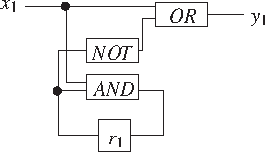
\includegraphics{exercise-2-1-1.pdf}
                        \caption*{\tiny from \cite[Exercise~2.1, p.~82]{model:checking}}
                    \end{figure}
            \end{columns}~\\

            \pause

            \vspace*{-2em}
            $TS_1 = (S_1, Act_1, \rightarrow_1, I_1, AP_1, L_1)$
            %$TS$ "uber $AP = \{ x_1, r_1, y_1 \}$
            \begin{center}
                \begin{tikzpicture}
                    \node[initial above, state]  (00) [label=below:\{$y_1$\}]                           {$x_1 = 0, r_1 = 0$};
                    \node[state]                 (01) [below=of 00, label=above:{\{$r_1$\}}]            {$x_1 = 0, r_1 = 1$};
                    \node[initial above, state]  (10) [right=of 00, label=below:{\{$x_1, y_1$\}}]       {$x_1 = 1, r_1 = 0$};
                    \node[state]                 (11) [below=of 10, label=above:{\{$x_1, r_1, y_1$\}}]  {$x_1 = 1, r_1 = 1$};

                    \path[->]    (00) edge[loop left]  (00)
                                                        edge[bend left]  (10)
                                             (10) edge[loop right] (10)
                                                        edge[bend left]  (00);
                \end{tikzpicture}
            \end{center}
        \end{Beispiel}

        \note{\begin{itemize}
                \item $S = Eval(x,r)$ alle m"oglichen Belegungen
                \item $Act$ irrelevant
                \item $I$ Belegungen mit gegebener Registerevaluation
                \item $AP$ alle Eingaben/Register/Ausgaben
                \item $L$ und $\rightarrow$ ergeben sich aus $S$ und boolescher Funktion
            \end{itemize}}
    }
\end{frame}



\def\schaltwerkinner{
    \node[initial below, state]  (01) [below=of 00, label=above:{\{$r_2$\}}]         {$x_2 = 0, r_2 = 1$};
    \node[initial below, state]  (11) [below=of 10, label=above:{\{$x_2,r_2,y_2$\}}] {$x_2 = 1, r_2 = 1$};

    \path[->]    (01) edge[loop left]  (01)
                                        edge[bend left]  (11)
                           (11) edge[loop right] (11)
                                        edge[bend left]  (01);
}

\newcommand{\schaltwerk}{
    \begin{center}
        \begin{tikzpicture}
        \schaltwerkinner
        \end{tikzpicture}
    \end{center}
}

\begin{frame}{Beispiele TS - Schaltwerk}
    \begin{Beispiel}[Exercise~2.1 a - TS von Schaltwerken (2)]
        \vspace*{-1em}
        \begin{columns}
            \column{0.45\textwidth}
                $y_2 = x_2 \land r_2$ \\
                $\delta_{r_2} = x_2 \lor r_2$\\[\baselineskip]

                Annahme (b): initial $r_2 = 1$

            \column{0.4\textwidth}
            \begin{figure}[H]
                    \centering
                    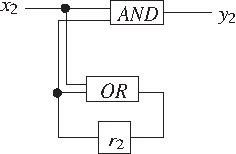
\includegraphics{exercise-2-1-2.pdf}
                    \caption*{\tiny from \cite[Exercise~2.1, p.~82]{model:checking}}
                \end{figure}
        \end{columns}~\\

        \pause

        \vspace*{-2em}
        $TS_2 = (S_2, Act_2, \rightarrow_2, I_2, AP_2, L_)$\vspace*{-1.5em}
        \begin{center}
            \begin{tikzpicture}
                \schaltwerkinner

                \node[state]                 (00) [label=above:{\{\}}]                           {$x_2 = 0, r_2 = 0$};
                \node[state]                 (10) [right=of 00, label=above:{\{$x_2$\}}]         {$x_2 = 1, r_2 = 0$};
            \end{tikzpicture}
        \end{center}
    \end{Beispiel}
\end{frame}



\begin{frame}{Paths und Traces - Beispiele}
    \begin{Beispiel}[Schaltwerk 2 aus Exercise 2.1]
        % \schaltwerk
        \begin{center}
            \begin{tikzpicture}
            \schaltwerkinner

            \node[thick, font=\bfseries] at ([yshift=-0.5cm,xshift=-0.5cm]01) {1};
            \node[thick, font=\bfseries] at ([yshift=-0.5cm,xshift=0.5cm]11) {2};
            \end{tikzpicture}
        \end{center}

        \vspace*{-\baselineskip}
        infinite Path Fragment:
        \begin{itemize}
            \item $\pi_1 = 12111\dots = 121^\omega$ \alert{initial, maximal}, also $\pi_1 \in \Paths(TS)$ \\
            \onslide<2->{$\trace(\pi_1) = \{r_2\}\{x_2,r_2,y_2\}\{r_2\}^\omega$}
            \item $\pi_2 = 221212\dots = 22(12)^\omega$ \alert{initial, maximal}, $\pi_2 \in \Paths(TS)$ \\
            \onslide<2->{$\trace(\pi_2) = \{x_2,r_2,y_2\}^2 \big(\{r_2\}\{x_2,r_2,y_2\}\big)^\omega$}
        \end{itemize}

        finite Path Fragment:
        \begin{itemize}
            \item $\hat{\pi}_1 = 111$ \alert{initial}
            \item $\hat{\pi}_2 = 2211$ \alert{initial}
        \end{itemize}
    \end{Beispiel}
\end{frame}



\begin{frame}
    \Huge\centering Beispielaufgaben
\end{frame}

\begin{frame}
    \frametitle{Exercise 3.5.}
    % TODO: add rest; Einordnung
    TS mit $AP = \{x=0, x>1\}$.  Formuliere als LT-Property $P$:
    \note{einorgnen: Invariante / Safety / Liveness}
    \begin{enumerate}[<+->]
        \renewcommand{\theenumi}{\alph{enumi}}
        \item \alert{false} \quad
                $P = \emptyset$
        \item \alert{am Anfang gilt: $x=0$} \quad
                $P = \big\{ A\sigma \; | \; \{x=0\} \in A \; \land \; \sigma \in (2^{AP})^\omega \big\}$
        \item \alert{am Anfang gilt: $x\neq 0$} \quad
                $P = \big\{ A\sigma \; | \; \{x>1\} \in A \; \land \; \sigma \in (2^{AP})^\omega \big\}$
        \item \alert{am Anfang ist $x=0$, aber irgendwann $x>1$} \quad \\
                $\begin{aligned}
                        P = &\big\{ A\sigma \; | \; \{x=0\} \in A \; \land \; \sigma \in (2^{AP})^\omega \big\} \\
                        &\cap \big\{ A_0 A_1 A_2 \dots \in (2^{AP})^\omega \; | \;
                                \exists i\geq 0.\; \{x>1\}\subseteq A_j\big\}
                        \end{aligned}$
        \item \alert{$x>1$ nur endlich oft} \quad
                $P = \big\{ A_0 A_1 A_2 \dots \in (2^{AP})^\omega \; | \;
                \exists i\geq 0.\; \forall j \geq i.\; \{x>1\}\not\subseteq A_j \big\}$
        \item \alert{$x>1$ unendlich oft} \quad
                $P = \big\{ A_0 A_1 A_2 \dots \in (2^{AP})^\omega \; | \;
                \forall i\geq 0.\; \exists j \geq i.\; \{x>1\}\subseteq A_j \big\}$
        \item --
        \item \alert{true} \quad
                $P = (2^{AP})^\omega$
    \end{enumerate}
\end{frame}

\begin{frame}[typeset second]{Exercise 3.6.}
    \only<second>{
        \defsafety
        \defliveness
    }

    \only<second:0>{
        \begin{enumerate}[<+->]
            \renewcommand{\theenumi}{\alph{enumi}}
            \item $P = \{ A_0 A_1 A_2 \dots \in (2^{AP})^\omega \; | \;
                    \forall i\geq0 A \not\in A_i \}$
                    \alert{Invariante}
            \item $P = \{ A_0 A_1 A_2 \dots \in (2^{AP})^\omega \; | \;
                    \exists ! \; i \geq 0. \; A \in A_i \}$ \\
                    \alert{in keiner bekannten Kategorie}
                    \begin{itemize}[<+->]
                        \item \alert{keine Liveness P.:} $\pref(P) \neq (2^{AP})^*$, da $\hat{\sigma} = \{A\}^2 \; \not\in \; \pref(P)$
                        \item \alert{keine Safety P.:} Sei z.\,B. $\sigma = A_0 A_1 A_2 \dots \in (2^{AP})^\omega \setminus P_{safe}$ ein Trace f"ur den gilt:
                            $\forall i\geq0.\; A \not\in A_i$ \\
                            Dann existiert kein Pr"afix von $\sigma$, welches sich zu einem Wort in $P$ verl"angern l"asst.
                        \item \alert{keine Invariante.:} trivial
                    \end{itemize}
            \item $\begin{aligned}[t]P = \{ A_0 A_1 A_2 \dots &\in (2^{AP})^\omega \; | \;
                    \forall i\geq0.\; \exists j \geq i.\; A\in A_j \quad \land \quad \\
                    &\forall i\geq0.\; \exists j \geq i.\; B\in A_j \}\end{aligned}$ \\
                    \alert{Liveness P.:} Anh"angen von $\Big(\{A\}\{B\}\Big)^\omega$
            \item $P = \big\{ A_0 A_1 A_2 \dots \; | \;
                    \forall i\geq0.\; (A\in A_i \Rightarrow (\exists j>i.\; B\in A_j)) \big\}$ \\
                    \alert{Liveness P.:} Anh"angen von $\{B\}^\omega$
        \end{enumerate}
    }
\end{frame}


\end{document}
